%!TeX root =  ../../thesis.tex

\section{Display}

Pro potřeby testeru byl vybrán standardní LCD displej se žlutým podsvícením o čtyřech řádcích po dvaceti znacích. Tento displej bude postačovat, jelikož je potřeba zobrazit menu, aby uživatel mohl vybrat typ kabelu dle koncových konektorů a následně výsledek testu, kterému jsou věnovány poslední dva řádky, na které se taky budou vypisovat chybová hlášení. V prvním řádku je vypsána verze programu a na poslední pozici bliká znak “\#”, který se objeví a zmizí vždy na jednu sekundu, z důvodu kontroly, že zařízení “nezamrzlo” a je možné jej bez problému použít.

\begin{figure}[H]
	\centering
	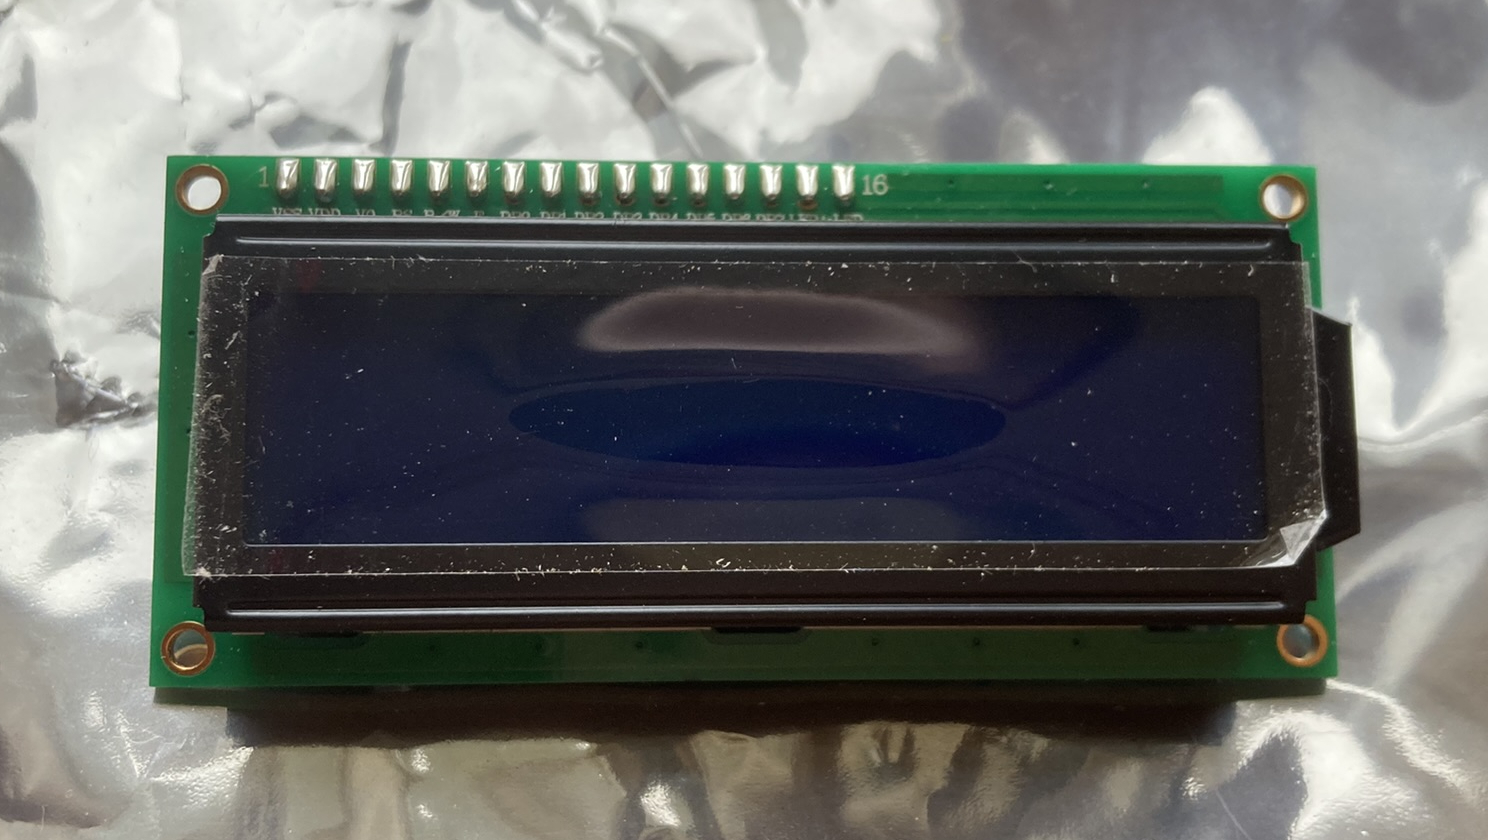
\includegraphics[width=0.9\textwidth]{pictures/display.jpeg}
    	\caption{Display}
   	\label{fig:displayHW}
\end{figure}

Na obrázku \ref{fig:displayHW} je displej, který sice není použitý pro tester, ale je to principiálně stejný displej a vlevo nahoře jsou vidět vrchní strany pinů, kterými se displej připojuje k Arduino nebo po případě k breadbordu.